% TODO (authors, M10): psi is both the digamma function (lines 56 to 235) and Chebyshev's function (lines 62 onwards); P_sigma prime piece vs P_a Poisson kernel vs P_n Gneiting; A_sigma vs A_h; G vs G_h. Choose distinct symbols.
% TODO (authors): chi_{-4} here, chi_4 in the cited theorem; 'quasi GGC' undefined; 'Thorin ladder of Volume I' has no matching object; figures fig_mu, fig_k not verified; status word for the approximate paragraph near n:thm:primes; Polya49 bib entry unchecked.
% 18 Nov 2026: sections nf:sec:four to nf:sec:gives added from Nick's Nakamura factorisation note (misc/reviews/nick-nakamura2/nakamura/nakamura_chapter.tex, new parts only), referee NAK2 (M1 to M9) and verification misc/vol3/verify/NAK2/results.md; figures fig/v3/nk2_fig_strip.pdf and nk2_fig_strip_thorin.pdf.
% Chapter 4 of Volume III: Nakamura's measure, positive definiteness and the Polya and Gneiting obstruction. Sources: misc/reviews/nick-volume3/vol3/ch2_nakamura.tex (ranges of STRUCTURE.md, Chapter 4), referee reports U02 (M1 to M9 and minors) and V3C (ch2 part), verification W5 (V17). Draft chart u=w^2/2 converted to the book's u=w^2 (N1), xi with Riemann's factor 1/2 (N3). 17 Nov 2026.
\label{n:ch:nakamura}

This chapter connects the quasi infinite divisibility of the completed zeta function, discovered by Nakamura, to the Thorin measures of Volumes I and II, and asks whether the classical sufficient conditions for positive definiteness (Pólya, Gneiting) can prove the positivity of the Thorin density. Pólya's criterion fails outright, and on RH Gneiting's fails for every Gaussian smoothing, because of the zeros themselves. The chapter is built on an unrefereed note of Polson (November 2026). Its statements are marked proved, computed, conditional or open. Results already proved in Volumes I and II are cited, not reproved.

Throughout, $\xi(s)=\frac12s(s-1)\pi^{-s/2}\Gamma(s/2)\zeta(s)$ is the book's completed function, $\Theta=\sup\re\rho$ over the zeros of $\zeta$, $c_\sigma=\xi'(\sigma)/\xi(\sigma)$, and $\Lambda(n)$ is the von Mangoldt function. For real $\sigma>\frac12$ and $v\in\R$ put
\begin{equation}\label{n:eq:k}
k_\sigma(v)=\frac1\pi\Big[\re\frac{\xi'}{\xi}(\sigma+iv)-c_\sigma\Big].
\end{equation}
This is the compensated density: the book's strip density $v_\sigma(v)=\re(\xi'/\xi)(\sigma+iv)$ of \eqref{eq:Ualpha}, minus its value $c_\sigma=v_\sigma(0)$ at the origin, divided by $\pi$. It is an even function with $k_\sigma(0)=0$, defined at every level $\sigma>\frac12$ and real analytic except at the ordinates of zeros with real part $\sigma$.

\section{Nakamura's theorems}\label{n:sec:nak}

A characteristic function $\hat\eta$ has a Lévy Khintchine form if
\begin{equation}\label{n:eq:lk}
\hat\eta(t)=\exp\Big[i\gamma t-\frac a2t^2+\int_{\R}\big(e^{itx}-1-itx\,\mathbf 1_{\{|x|\le1\}}\big)\nu(dx)\Big].
\end{equation}
The law is infinitely divisible when $a\ge0$ and $\nu\ge0$. It is quasi infinitely divisible when \eqref{n:eq:lk} holds with a signed measure $\nu$ with $\int(x^2\wedge1)\,|\nu|(dx)<\infty$, equivalently when $\hat\eta$ is a quotient of two infinitely divisible characteristic functions (Lindner, Pan and Sato \cite{LPS18}; see Proposition~\ref{sb:prop:qid}). Following Nakamura, a law is called pretended infinitely divisible when \eqref{n:eq:lk} holds with a signed $\nu$ and the integrability of $|\nu|$ is dropped.

\begin{theorem}[Nakamura \cite{Nakamura15}]\label{n:thm:nak}
Put $\Xi_\sigma(t)=\xi(\sigma-it)/\xi(\sigma)$.
\begin{enumerate}
\item For every real $\sigma$, $\Xi_\sigma$ is a characteristic function.
\item $\Xi_\sigma$ is pretended infinitely divisible for every $\sigma\in(\frac12,1)$ if and only if RH holds. Under RH, at each such level,
\[
\Xi_\sigma(t)=\exp\Big[\int_0^\infty(e^{itx}-1)\nu_\sigma(dx)\Big],\qquad \nu_\sigma(dx)=-\sum_{\gamma>0}\frac{2\cos(\gamma x)}{x\,e^{(\sigma-1/2)x}}\,dx,
\]
where the zeros are summed in conjugate pairs inside the exponent, which fixes the convergence.
\item For $\sigma=1$, $\Xi_\sigma$ is pretended infinitely divisible, unconditionally.
\item For $\sigma>1$, $\Xi_\sigma$ is quasi infinitely divisible and not infinitely divisible, with
\begin{equation}\label{n:eq:naknu}
\nu_\sigma(dx)=\frac{dx}{x\,e^{\sigma x}(1-e^{-2x})}-\frac{(1+e^x)\,dx}{x\,e^{\sigma x}}+\sum_{n\ge2}\frac{\Lambda(n)n^{-\sigma}}{\log n}\,\delta_{\log n}(dx).
\end{equation}
\end{enumerate}
\end{theorem}

The quantifier in part 2 matters. The converse uses a zero at the level where it sits, so it is a statement about the whole family of levels in $(\frac12,1)$, not about one fixed level. A representation at one level $\sigma>\Theta$ is compatible with zeros to the left of $\sigma$ (Theorem~\ref{thm:poisson}). The three pieces of \eqref{n:eq:naknu} come from $\Gamma(s/2)$, from the factor $s(s-1)$ and from the Euler product. For $\sigma>1$ this is the signed Lévy measure of Proposition~\ref{sb:prop:qid}, and the compensated form is the L\'evy form stated before it, which at $\sigma=1$ is Proposition~\ref{bp:prop:levy}. Nakamura and Suzuki \cite{NakamuraSuzuki23} treat the infinitely divisible side of the same circle of ideas.

\section{One measure for every level}\label{n:sec:oneline}

Every term of \eqref{n:eq:naknu} has the form $e^{-\sigma x}\mu(dx)/x$ with one measure $\mu$ that does not depend on $\sigma$.

\begin{proposition}[proved]\label{n:prop:oneline}
Let
\begin{equation}\label{n:eq:mu}
\mu(dx)=\sum_{n\ge2}\Lambda(n)\,\delta_{\log n}(dx)+\frac{dx}{1-e^{-2x}}-(1+e^x)\,dx\qquad(x>0).
\end{equation}
Then for $\re s>1$
\begin{equation}\label{n:eq:second}
(\log\xi)''(s)=\int_0^\infty x\,e^{-sx}\,\mu(dx),
\end{equation}
and Nakamura's measure is $\nu_\sigma(dx)=e^{-\sigma x}\mu(dx)/x$. Write $m_\sigma(dx)=e^{-\sigma x}\mu(dx)$.
\end{proposition}

\begin{proof}
Logarithmic differentiation gives $\frac{\xi'}\xi(s)=\frac1s+\frac1{s-1}-\frac12\log\pi+\frac12\psi(\frac s2)+\frac{\zeta'}{\zeta}(s)$, with $\psi=\Gamma'/\Gamma$. Differentiate once more and write each term as a Laplace transform of $x\mu(dx)$. For $\re s>1$, $-s^{-2}=-\int_0^\infty xe^{-sx}dx$ and $-(s-1)^{-2}=-\int_0^\infty xe^xe^{-sx}dx$. From $\psi'(z)=\int_0^\infty te^{-zt}(1-e^{-t})^{-1}dt$ and $t=2x$, $\frac14\psi'(\frac s2)=\int_0^\infty xe^{-sx}(1-e^{-2x})^{-1}dx$. Finally $(\zeta'/\zeta)'(s)=\sum_n\Lambda(n)\log n\;n^{-s}=\int_0^\infty xe^{-sx}\sum_n\Lambda(n)\delta_{\log n}(dx)$. The sum of the four terms is \eqref{n:eq:second}, and each piece of \eqref{n:eq:naknu} is $e^{-\sigma x}/x$ times the corresponding piece of $\mu$, because $\Lambda(n)/\log n=\Lambda(n)/x$ at $x=\log n$.
\end{proof}

Integrating \eqref{n:eq:second} twice in $s$ recovers Nakamura's form, the two constants being the normalisation $\Xi_\sigma(0)=1$ and the drift. All levels $\sigma>1$ share one measure, tilted by $e^{-\sigma x}$.

\begin{corollary}[proved]\label{n:cor:sign}
With $\psi(X)=\sum_{n\le X}\Lambda(n)$, and using $1/(1-e^{-2x})-1=1/(e^{2x}-1)$,
\begin{equation}\label{n:eq:split}
\mu=d\big(\psi(e^x)-e^x\big)+\frac{dx}{e^{2x}-1}.
\end{equation}
The gamma factor and the factor $s$ together give the positive density $1/(e^{2x}-1)$. The negative term $-e^x\,dx$ comes from the factor $s-1$ of $\xi$, which cancels the pole of $\zeta$ at $s=1$, and it is the main term of the prime number theorem. Hence $\mu$ is signed only through the prime remainder $\Delta(X)=\psi(X)-X$.
\end{corollary}

The decomposition \eqref{n:eq:split} is not the minimal one: the Jordan negative part of $m_\sigma$ is smaller, because the archimedean density $1/(e^{2x}-1)$ offsets part of the pole density. Figure~\ref{n:fig:mu} shows the three parts of $m_\sigma$ at $\sigma=2$.

\begin{figure}[t]
\centering
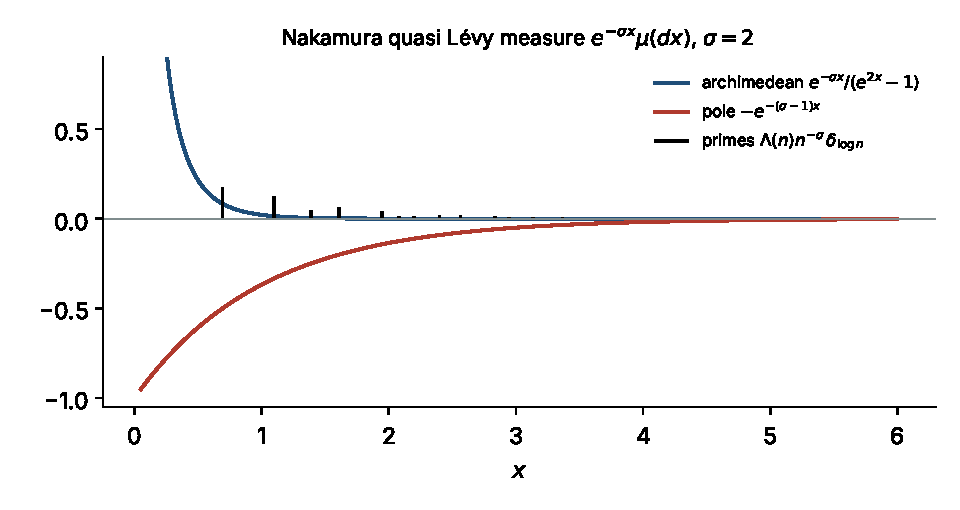
\includegraphics[width=\textwidth]{fig/v3/fig_mu.pdf}
\caption{Nakamura's measure tilted to level $\sigma=2$: the archimedean density $e^{-\sigma x}/(e^{2x}-1)$, the negative pole density $-e^{-(\sigma-1)x}$, and the prime atoms $\Lambda(n)n^{-\sigma}$ at $x=\log n$ (computed).}
\label{n:fig:mu}
\end{figure}

\section{The Thorin form and the extended GGC}\label{n:sec:thorin}

For $\sigma>1$ and $w\ge0$, the L\'evy form stated before Proposition~\ref{sb:prop:qid} (at $\sigma=1$, Proposition~\ref{bp:prop:levy}) gives the compensated form
\begin{equation}\label{n:eq:comp}
\log\frac{\xi(\sigma+w)}{\xi(\sigma)}=w\,c_\sigma+\int_0^\infty\big(e^{-wx}-1+wx\big)\frac{m_\sigma(dx)}x ,
\end{equation}
with absolutely convergent integral. The sine squared lemma \eqref{eq:sin2}, which is a linear map from compensated exponentials to logarithmic kernels, carries \eqref{n:eq:comp} to the Thorin side. For a measure $m$ put
\[
\mathcal T[m](dz)=\Big(\int_0^\infty\frac{1-\cos(x\sqrt z)}{2\pi\sqrt z}\,m(dx)\Big)dz .
\]
$\mathcal T$ is linear, and $m\ge0$ implies $\mathcal T[m]\ge0$. A difference of Lévy measures goes to a difference of Thorin measures.

\begin{theorem}[proved]\label{n:thm:thorin}
Let $\sigma>1$, $u\ge0$ and $w=\sqrt u$. Then
\begin{equation}\label{n:eq:thorin}
\frac{\xi(\sigma)}{\xi(\sigma+w)}\,e^{wc_\sigma}=\exp\Big(-\int_0^\infty\log\Big(1+\frac uz\Big)U^c_\sigma(dz)\Big),\qquad U^c_\sigma=\mathcal T[m_\sigma],
\end{equation}
and in the chart $z=v^2$ the signed measure $U^c_\sigma$ has the density $k_\sigma(v)\,dv$ of \eqref{n:eq:k}.
\end{theorem}

\begin{proof}
Negate \eqref{n:eq:comp}, insert \eqref{eq:sin2} for each $x$ and exchange the integrals. On the archimedean part and on the primes the integrands have one sign (Tonelli), and on the pole part both integrals converge absolutely. For the density define $G(s)=\int_0^\infty(e^{-\sigma x}-e^{-sx})\mu(dx)$ for $\re s\ge\sigma$. The integral converges because $e^{-\sigma x}-e^{-sx}=O(x)$ at $0$. Then $G(\sigma)=0$ and $G'(s)=(\log\xi)''(s)$ by \eqref{n:eq:second}, so $G(s)=\frac{\xi'}\xi(s)-c_\sigma$ (the boundary line $\re s=\sigma$ is reached by continuity). Taking $s=\sigma+iv$ and real parts, $\int_0^\infty(1-\cos vx)\,m_\sigma(dx)=\pi k_\sigma(v)$, and the kernel of $\mathcal T$ at $z=v^2$ turns this into $k_\sigma(v)\,dv$.
\end{proof}

Theorem~\ref{n:thm:thorin} is the compensated form of Theorem~\ref{thm:poisson}: the compensator $e^{wc_\sigma}$ is the stable factor with drift $b_\sigma=c_\sigma$ of Proposition~\ref{bp:prop:valpha}, and $U^c_\sigma$ is the Thorin measure of $T^\circ_\sigma$ there. Positivity of $k_\sigma$ for every $\sigma\ge1$, strictly, is Proposition~\ref{bp:prop:valpha} (ball arithmetic and the zero counts of \cite{HSW22}).

\subsection{The pieces}

With $\lambda=v\ge0$, applying $\mathcal T$ to the three parts of $m_\sigma$ gives, for $\sigma>1$,
\begin{equation}\label{n:eq:pieces}
\pi k_\sigma(v)=P_\sigma(v)+A_\sigma(v)-R_\sigma(v),
\end{equation}
where
\begin{align*}
P_\sigma(v)&=\sum_{n\ge2}\Lambda(n)n^{-\sigma}\big(1-\cos(v\log n)\big)=\re\frac{\zeta'}{\zeta}(\sigma+iv)-\frac{\zeta'}{\zeta}(\sigma),\\
A_\sigma(v)&=\int_0^\infty\frac{(1-\cos vx)e^{-\sigma x}}{e^{2x}-1}\,dx=\frac12\Big[\re\psi\Big(\frac{\sigma+iv}2\Big)-\psi\Big(\frac\sigma2\Big)\Big]-\frac{v^2}{\sigma(\sigma^2+v^2)},\\
R_\sigma(v)&=\int_0^\infty(1-\cos vx)e^{-(\sigma-1)x}\,dx=\frac{v^2}{(\sigma-1)\big((\sigma-1)^2+v^2\big)} .
\end{align*}
Here $P_\sigma,A_\sigma\ge0$ because their measures are, $R_\sigma\le1/(\sigma-1)$, and $A_\sigma(v)=\frac12\log v+O_\sigma(1)$. Nakamura's quasi infinite divisibility becomes a quasi GGC, a signed Thorin measure $U^c_\sigma=U^+-U^-$.

\subsection{The extended GGC}

Bondesson's extended GGC class \cite{Bondesson} consists of the laws on $\R$ with characteristic function $\exp\big(ibt-\frac c2t^2+\int_{\R\setminus\{0\}}[\log\frac v{v-it}-\frac{itv}{1+v^2}]K(dv)\big)$, $K\ge0$.

\begin{theorem}[proved]\label{n:thm:eggc}
Let $\sigma>1$ and let $Y_\sigma$ have Laplace transform \eqref{n:eq:thorin}, as a genuine random variable whenever $k_\sigma\ge0$ (this holds for every $\sigma\ge1$, Proposition~\ref{bp:prop:valpha}). Let $N\sim N(0,1)$ be independent and $X_\sigma=\sqrt{2Y_\sigma}\,N$. Then
\begin{equation}\label{n:eq:eggc}
\E\,e^{itX_\sigma}=\frac{\xi(\sigma)}{\xi(\sigma+|t|)}\,e^{|t|c_\sigma}
=\exp\Big(\mathrm{PV}\!\!\int_{\R}\log\frac{v}{v-it}\;k_\sigma(v)\,dv\Big),
\end{equation}
where the principal value is symmetric about $v=0$, equivalently the integrand carries the compensator $-itv/(1+v^2)$.
\end{theorem}

\begin{proof}
$\E e^{itX_\sigma}=\E e^{-t^2Y_\sigma}$, which is \eqref{n:eq:thorin} at $u=t^2$. With $z=v^2$ the exponent is $-\int_0^\infty\log(1+t^2/v^2)k_\sigma(v)\,dv$, and $-\log(1+t^2/v^2)=\log\frac v{v-it}+\log\frac v{v+it}$ with $k_\sigma$ even. The imaginary part of $\log\frac v{v-it}$ is of order $t/v$ and $k_\sigma(v)$ grows like $\frac1{2\pi}\log v$, so the integral over a half line diverges, and only the symmetric pairing converges.
\end{proof}

The variable $X_\sigma$ is a symmetric extended GGC, in particular infinitely divisible, exactly when $k_\sigma\ge0$ (the converse direction uses the uniqueness of the representation).

\section{The zero side}\label{n:sec:zeros}

By the Hadamard product, $\frac{\xi'}{\xi}(s)=\sum_\rho\frac1{s-\rho}$, with the zeros paired with their conjugates, so for every $\sigma>\frac12$ and every $v$ with $\sigma+iv$ not a zero
\begin{equation}\label{n:eq:kzero}
k_\sigma(v)+\frac{c_\sigma}\pi=\sum_\rho P_{\sigma-\beta}(v-\gamma),\qquad P_a(x)=\frac{a}{\pi(a^2+x^2)},\quad\rho=\beta+i\gamma,
\end{equation}
the series converging absolutely. This is Proposition~\ref{prop:struct}. For $\sigma>\Theta$ every width $\sigma-\beta$ is positive: $k_\sigma$ is Poisson smoothed zeros minus the constant $c_\sigma/\pi$. A zero with $\beta>\sigma$ contributes the negative kernel $P_{\sigma-\beta}=-P_{\beta-\sigma}$, of size $1/(\pi(\beta-\sigma))$ at $v=\gamma$. Under RH all widths equal $\sigma-\frac12$, $c_\sigma\to0$, and $k_\sigma(v)\,dv\to\sum_{\gamma>0}\delta_\gamma$ vaguely on $v>0$ as $\sigma\downarrow\frac12$. In the chart $z=v^2$ this is the level one half Thorin measure $\sum_{\gamma>0}\delta_{\gamma^2}$ of Volumes I and II, with multiplicity.

The function $u\mapsto\xi(\sigma)/\xi(\sigma+\sqrt u)$ is the Laplace transform of a GGC if and only if $\sigma\ge\Theta$ (Theorem~\ref{thm:poisson}), and it is one at every level of $(\frac12,1)$ if and only if RH holds. The sign of $k_\sigma$ on one line is a separate matter. Figure~\ref{n:fig:k} shows $k_\sigma$ above and inside the strip, where the bumps sharpen at the ordinates $\gamma$.

\begin{figure}[t]
\centering
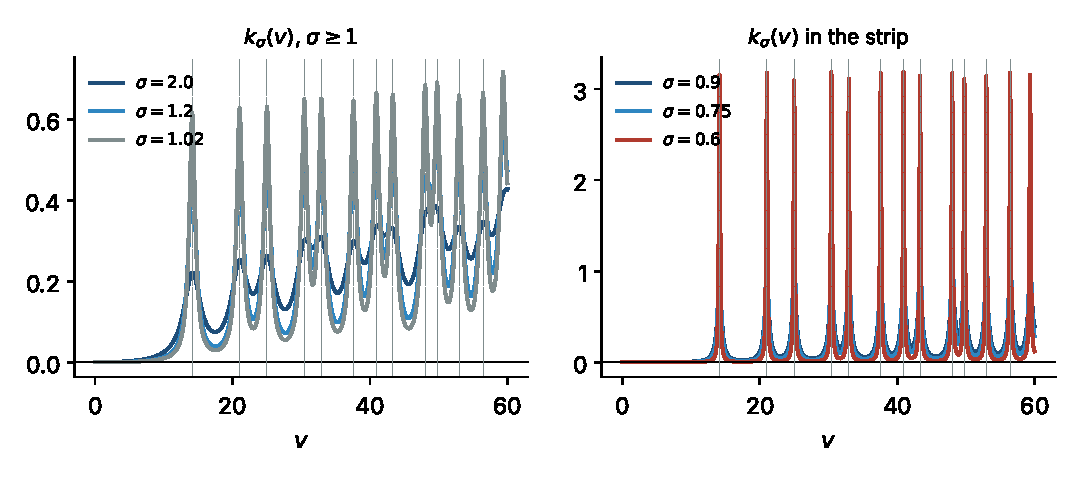
\includegraphics[width=\textwidth]{fig/v3/fig_k.pdf}
\caption{The density $k_\sigma(v)$ computed from $\zeta'/\zeta$ and $\psi$. Dotted lines mark the first twelve zero ordinates. Left: $\sigma=2,1.2,1.02$. Right: $\sigma=0.9,0.75,0.6$ (computed).}
\label{n:fig:k}
\end{figure}

\section{Positivity as positive definiteness}\label{n:sec:bochner}

Define for $\sigma>1$ the tails of the tilted measure, and extend $M_2$ to an even function on $\R$:
\[
M_1(x)=\int_x^\infty m_\sigma(dy),\qquad M_2(x)=\int_x^\infty(y-x)\,m_\sigma(dy),\qquad x>0 .
\]
Both tails are finite, $M_2'=-M_1$, $M_2''=m_\sigma$ away from the origin, and $M_2(0)=(\log\xi)''(\sigma)>0$.

\begin{theorem}[proved]\label{n:thm:bochner}
For $\sigma>1$ and $v>0$,
\begin{equation}\label{n:eq:kM2}
\pi k_\sigma(v)=\int_0^\infty(1-\cos vx)\,m_\sigma(dx)=v^2\int_0^\infty\cos(vx)M_2(x)\,dx=\frac{v^2}{2}\widehat{M_2}(v).
\end{equation}
Consequently $k_\sigma\ge0$ if and only if $M_2$ is a positive definite function on $\R$.
\end{theorem}

\begin{proof}
Put $g(x)=1-\cos vx$, so $g(0)=g'(0)=0$ and $g''=v^2\cos vx$. Integrating by parts twice, $\int_0^\infty g\,dM_2'=[gM_2'-g'M_2]_0^\infty+\int_0^\infty g''M_2\,dx$. The boundary terms vanish at $0$ because $g(x)M_1(x)=O(x^2\log(1/x))$ and $g'(0)=0$, and at infinity because $M_1$ and $M_2$ decay exponentially for $\sigma>1$. This is \eqref{n:eq:kM2}. The function $M_2$ is continuous, even and integrable, so by Bochner's theorem it is positive definite if and only if $\widehat{M_2}\ge0$, which is $k_\sigma\ge0$ on $v>0$ (at $v=0$, $k_\sigma$ vanishes, and $\widehat{M_2}(0)\ge0$ follows by continuity).
\end{proof}

For $\sigma>1$ this is known to hold (Proposition~\ref{bp:prop:valpha}), so the question has content only through its structure: the positivity of $k_\sigma$ is a Pólya type problem for the twice integrated tail of a signed measure. It is the minimum of $v_\sigma$ at the origin, the theorem of Lagarias \cite{Lagarias} recalled in Section~\ref{n:sec:path}.

\section{The criteria of Pólya and Gneiting}\label{n:sec:gneiting}

Let $\varphi:[0,\infty)\to\R$ be continuous with $\varphi(0)=1$ and $\varphi(t)\to0$ as $t\to\infty$.

\begin{theorem}[Pólya \cite{Polya49}]
If $\varphi$ is convex and nonincreasing on $(0,\infty)$, then $\varphi(|t|)$ is a characteristic function.
\end{theorem}

\begin{theorem}[Gneiting \cite{Gneiting00}]
Let $\varphi$ be twice continuously differentiable on $(0,\infty)$. If $t\mapsto t^{-1}\big(\sqrt t\,\varphi''(\sqrt t)-\varphi'(\sqrt t)\big)$ is convex on $(0,\infty)$, then $\varphi(|t|)$ is the characteristic function of an absolutely continuous law.
\end{theorem}

Gneiting's criterion allows concave stretches and smooth behaviour at the origin, which Pólya's excludes. His criteria of type $P_n$ \cite{Gneiting01} ask for convexity of a higher derivative after the change $t\mapsto\sqrt t$. We treat only the two displayed criteria. For $\varphi=M_2/M_2(0)$ we have $\varphi'=-M_1/M_2(0)$, $\varphi''=m_\sigma/M_2(0)$, so each criterion is a condition on Nakamura's measure.

Split $m_\sigma=m^{\rm arch}_\sigma+m^\Delta_\sigma$ by \eqref{n:eq:split}, with $m^{\rm arch}_\sigma=e^{-\sigma x}dx/(e^{2x}-1)$ and $m^\Delta_\sigma=e^{-\sigma x}d(\psi(e^x)-e^x)$.

\begin{proposition}[proved]\label{n:prop:gneiting}
Let $\sigma>1$.
\begin{enumerate}
\item The second tail $M_2^{\rm arch}=\sum_{j\ge1}e^{-(\sigma+2j)x}/(\sigma+2j)^2$ is convex and decreasing, so positive definite, and $\mathcal T[m_\sigma^{\rm arch}]\ge0$. This holds for every $\sigma>0$.
\item The prime atoms alone give a convex, positive definite second tail, a sum of triangles $a_n(\log n-|x|)_+$ with $a_n=\Lambda(n)n^{-\sigma}$.
\item $M_2$ is not convex. Between consecutive values $\log n$ its second derivative is $e^{-\sigma x}\big(1/(e^{2x}-1)-e^x\big)$, negative exactly when $e^{3x}-e^x>1$, that is for $x>\log y_*\approx0.281$, where $y_*\approx1.3247$ is the real root of $y^3=y+1$. Pólya's criterion does not apply.
\item Replace the primes by a smooth density $\ell(x)\,dx$, with finite tails, $M_2(0)>0$ and the differentiability that Gneiting's theorem needs. If $\ell(x)=e^x$ the pole cancels, $M_2=M_2^{\rm arch}$, and both criteria apply. For general $\ell$, positivity follows when Gneiting's function is convex.
\item For the true primes $m_\sigma$ has atoms. In the variable $t=x^2$ an atom of mass $a_n$ at $x=\log n$ contributes $2a_n\,\delta(t-\log^2n)/M_2(0)$ to Gneiting's function, a positive atom, which is not a convex function. The criterion does not apply directly.
\end{enumerate}
\end{proposition}

These are sufficient conditions, not an equivalent form of the positivity. The obstruction is entirely in the prime remainder: on average the primes cancel the pole and leave a positive measure, and the question is whether the fluctuations of $\psi(X)-X$ can drive the cosine transform negative.

\section{The condition on the primes}\label{n:sec:primes}

\begin{theorem}[proved]\label{n:thm:primes}
Let $\sigma>\Theta$, and read $\int_0^\infty e^{-\sigma x}d\Delta(e^x)$ as an improper Stieltjes integral, which converges. Then $k_\sigma\ge0$ if and only if, for every $v>0$,
\begin{equation}\label{n:eq:primecond}
\int_0^\infty(1-\cos vx)\,e^{-\sigma x}\,d\Delta(e^x)\;\ge\;-A_\sigma(v).
\end{equation}
For $\sigma>1$ this is $P_\sigma+A_\sigma\ge R_\sigma$, that is
\begin{multline}\label{n:eq:primecond2}
\re\frac{\zeta'}{\zeta}(\sigma+iv)-\frac{\zeta'}{\zeta}(\sigma)+\frac12\Big[\re\psi\Big(\frac{\sigma+iv}2\Big)-\psi\Big(\frac\sigma2\Big)\Big]\\ \ge\frac{v^2}{\sigma(\sigma^2+v^2)}+\frac{v^2}{(\sigma-1)\big((\sigma-1)^2+v^2\big)} .
\end{multline}
\end{theorem}

\begin{proof}
By partial integration $\int^\infty e^{-sx}d\Delta(e^x)$ converges for $\re s>\Theta$, since $\Delta(X)=O(X^{\Theta+\varepsilon})$ (Landau's theorem identifies $\Theta$ with the exponent of $\Delta$). A convergent Laplace Stieltjes integral is analytic to the right of its abscissa of convergence, so the identity \eqref{n:eq:second} continues from $\re s>1$ to $\re s>\Theta$, and so does the computation of $G$ in the proof of Theorem~\ref{n:thm:thorin}. By \eqref{n:eq:split}, $\pi k_\sigma(v)=\int(1-\cos vx)e^{-\sigma x}d\Delta(e^x)+A_\sigma(v)$, which is \eqref{n:eq:primecond}. For $\sigma>1$ the first term is $P_\sigma-R_\sigma$ by \eqref{n:eq:pieces}, and the $s$ factor piece $v^2/(\sigma(\sigma^2+v^2))$ of $A_\sigma$ goes to the right side.
\end{proof}

In words, the cosine transform of the prime remainder may be negative, but never by more than the archimedean term $A_\sigma$. Near $\sigma=1$ the archimedean term wins only for $v\ge V(\sigma)$ with $\log V(\sigma)=2/(\sigma-1)+O(1)$, so the primes carry the inequality over an exponentially long window, on which $P_\sigma(v)\approx\frac1{\sigma-1}+\re\frac{\zeta'}{\zeta}(1+iv)$. The inequality then requires $\re\frac{\zeta'}\zeta(1+iv)$ to be bounded below there, a quantitative form of $\zeta(1+iv)\ne0$.

\subsection{Small and large frequencies}

\begin{proposition}[proved]\label{n:prop:origin}
For every real $\sigma>\frac12$, unconditionally,
\[
k_\sigma(v)=-\frac{v^2}{2\pi}\Big(\frac{\xi'}{\xi}\Big)''(\sigma)+O(v^4),\qquad\Big(\frac{\xi'}{\xi}\Big)''(\sigma)<0,
\]
so $k_\sigma>0$ on a punctured neighbourhood of $v=0$. At $\sigma=\frac12$ the second derivative vanishes.
\end{proposition}

\begin{proof}
The expansion is Taylor's theorem for the real part of the analytic function $\xi'/\xi$ at the real point $\sigma$. For the sign use $(\xi'/\xi)''(\sigma)=\sum_\rho2(\sigma-\rho)^{-3}$. A conjugate pair $\beta\pm i\gamma$ contributes $4f(b)$ with $b=\sigma-\beta$, $f(b)=b(b^2-3\gamma^2)/(b^2+\gamma^2)^3$ and $f'(b)=-3(b^4-6b^2\gamma^2+\gamma^4)/(b^2+\gamma^2)^4$. For $1\le\sigma<\sqrt3\gamma_1\approx24.48$ every $b$ lies in $(0,\sigma)$, so $b^2<3\gamma^2$ and every pair contributes a negative amount. For $\sigma\ge24$ write $(\xi'/\xi)''(\sigma)=\frac2{\sigma^3}+\frac2{(\sigma-1)^3}+\frac18\psi''(\frac\sigma2)-\sum_n\Lambda(n)\log^2n\,n^{-\sigma}$. Since $\psi''(y)\le-y^{-2}$, the gamma term is at most $-1/(2\sigma^2)$, which exceeds $2\sigma^{-3}+2(\sigma-1)^{-3}$ in size once $\sigma\ge24$, and the prime term is negative. For $\frac12<\sigma<1$ the widths may have either sign if RH fails. The function $f$ is odd and strictly decreasing on $|b|<(\sqrt2-1)\gamma$, and $\gamma\ge\gamma_1>14$. By the functional equation the zeros come in quadruples $\beta\pm i\gamma$, $1-\beta\pm i\gamma$, with widths $b_1=\sigma-\beta$ and $b_2=\sigma-1+\beta$ in $(-1,1)$ and $b_1+b_2=2\sigma-1>0$. Hence $f(b_1)+f(b_2)=f(b_1)-f(-b_2)<0$. On the critical line $b_1=b_2=\sigma-\frac12>0$ and the conclusion holds. At $\sigma=\frac12$, $\xi'/\xi$ is odd about $\frac12$.
\end{proof}

At small $v$, $P_\sigma(v)\approx\frac{v^2}2\sum\Lambda(n)\log^2n\,n^{-\sigma}$, and this sum is $2/(\sigma-1)^3+O(1)$ as $\sigma\downarrow1$, which cancels the pole term $R_\sigma(v)\approx v^2/(\sigma-1)^3$: this is Chebyshev's $\psi(X)\sim X$ in Thorin form. At large $v$ the archimedean term wins on its own, as $A_\sigma(v)=\frac12\log v+O_\sigma(1)$, $P_\sigma\ge0$ and $R_\sigma\le\frac1{\sigma-1}$ (proved, by Stirling's formula). A uniform and strict statement for every $\sigma\ge1$ is Proposition~\ref{bp:prop:valpha}, and for the minimum at the origin on RH, for every $\sigma>\frac12$, Theorem~\ref{yo:thm:coercive}.

\section{Gneiting's criterion is obstructed by the zeros}\label{n:sec:obstruct}

The prime atoms can be removed without loss. Let $G_h$ be the centred Gaussian density of variance $h^2$.

\begin{lemma}[proved]\label{n:lem:gauss}
For $\sigma>1$ and every $h>0$, $M_2$ is positive definite if and only if $M_2*G_h$ is positive definite, and $\pi k_\sigma(v)e^{-h^2v^2/2}=\frac{v^2}2\widehat{M_2*G_h}(v)$.
\end{lemma}

\begin{proof}
$\widehat{G_h}(v)=e^{-h^2v^2/2}>0$, so $\widehat{M_2*G_h}=\widehat{M_2}\,\widehat{G_h}$ has the sign of $\widehat{M_2}$. Combine with Theorem~\ref{n:thm:bochner}.
\end{proof}

The smoothed function $\varphi_h=(M_2*G_h)/(M_2*G_h)(0)$ is smooth, and the denominator is positive by Theorem~\ref{n:thm:bochner} and Proposition~\ref{bp:prop:valpha}. The two criteria can be tested on it, and they fail.

\begin{theorem}[conditional (RH)]\label{n:thm:obstruct}
Assume RH and let $\sigma>1$, $h>0$. Then Gneiting's condition fails for $\varphi_h$, and so does Pólya's. More precisely there are arbitrarily large $x$ with $N_h(x)=x\varphi_h''(x)-\varphi_h'(x)<0$ and $\varphi_h''(x)<0$.
\end{theorem}

\begin{proof}
A convex function on $(0,\infty)$ that tends to $0$ at infinity is nonnegative, so Gneiting's condition forces $N_h\ge0$ on $(0,\infty)$, and Pólya's forces $\varphi_h''\ge0$. Put $F=M_2$, as an even function, and $a=\sigma-\frac12>0$. The even extension of $m_\sigma$ has density $\sim1/(2|x|)$ at $0$, so it is not a locally finite measure, but $F$ is continuous and $F''$ is a distribution that equals $m_\sigma$ away from $0$. By the explicit formula $\psi(e^x)-e^x=-\sum_\rho e^{\rho x}/\rho-\log2\pi-\frac12\log(1-e^{-2x})$, the last term cancels the archimedean density on differentiation, and on $(0,\infty)$, as distributions, $F''(x)=-\sum_\gamma e^{(-a+i\gamma)x}$, summed over all ordinates $\gamma$ with multiplicity and without any claim of pointwise convergence. Take a smooth cutoff vanishing near $0$ and equal to $1$ for $x\ge2$. The remaining part of $F''$ is a distribution of finite order supported in a bounded interval, plus the reflected part, and its Gaussian convolution contributes $O(e^{-x^2/(Ch^2)})$ at large positive $x$, with the same bound after finitely many differentiations. Gaussian smoothing multiplies each exponential by $e^{(-a+i\gamma)^2h^2/2}$, whose modulus decays like $e^{-h^2\gamma^2/2}$, while the zeros are polynomially many, so every differentiated series converges absolutely. Hence
\begin{multline*}
(F*G_h)''(x)=-e^{-ax}A_h(x)+O(e^{-x^2/(Ch^2)}),\\ A_h(x)=2\re\sum_{\gamma>0}m_\gamma e^{(-a+i\gamma)^2h^2/2}e^{i\gamma x},
\end{multline*}
with $m_\gamma$ the multiplicity. $A_h$ is a nonzero almost periodic function of mean zero (every frequency has a nonzero coefficient, and equal ordinates add), so there are $\delta>0$ and arbitrarily large $x$ with $A_h(x)\ge\delta$. Integrating the same series, $-(F*G_h)'(x)=e^{-ax}B_h(x)+O(e^{-x^2/(Ch^2)})$ with $B_h$ bounded, since every denominator $a-i\gamma$ is nonzero. At those $x$, $N_h(x)\propto e^{-ax}\big(-xA_h(x)+B_h(x)\big)<0$ once $x>\sup|B_h|/\delta$, and $\varphi_h''(x)<0$.
\end{proof}

Pólya's failure has a shorter proof that needs no zeros: a nonconstant even smooth function has $\varphi_h'(0)=0$, and a convex function with this property cannot decrease to zero. The zeros are needed for Gneiting's condition. RH is used only to fix the single exponent $-a$ in the oscillating term; without it the zeros of largest real part would play the same role, but the argument is then no longer a one line statement and we do not pursue it.

The theorem rules out the two named criteria for Gaussian smoothings, and says nothing about other kernels, about the criteria of type $P_n$ or about other derivative conditions. What it shows is that after the prime number theorem cancels the pole, what remains of Nakamura's measure is an oscillation at the frequencies $\gamma$, so a condition on the sign of a fixed combination of derivatives of $\varphi$ at large $x$ cannot hold. Positive definiteness of $M_2$ is a global property, the minimum of $v_\sigma$ at the origin (nonnegativity of $\hat M_2$), which these local convexity conditions cannot see. A computation in double precision, with the prime atoms up to $2\times10^5$ in closed form, confirms the failure at small $x$ (computed): for $\sigma=2,3$ and $h=0.05,0.1,0.25$, the function $N_h$, computed for $\varphi_h$ normalised by division by $(M_2*G_h)(0)$, is negative for $x$ near $0.85$ to $1.04$, between $\log2$ and $\log3$. The size of the minimum depends on the normalisation and we give no values.

\section{Xi plus pole equals primes plus Gamma}\label{nf:sec:four}

The sections that follow split Nakamura's representation for $\sigma>1$ into its factors, read the factorisation on densities, on Wald couples and on hitting times, and continue it into the strip. Nakamura's measure itself \cite{Nakamura15} is Theorem~\ref{n:thm:nak} and Proposition~\ref{sb:prop:qid}, and the Thorin pieces are \eqref{n:eq:pieces}. What is new here is the identity in law between four independent variables, the first order reading of Riemann's kernel, the classification of the factors by side, and the strip law. These parts are from an unrefereed note of Polson (November 2026), in the notation of this chapter. We have not found the identity in law or the strip identity in the literature.

Notation. For $\sigma>0$ the book's $V_\sigma$ has $\E\,e^{wV_\sigma}=\xi(\sigma+w)/\xi(\sigma)$ (Proposition~\ref{bp:prop:valpha}), so the variable with characteristic function $\Xi_\sigma(t)=\xi(\sigma-it)/\xi(\sigma)$ is $\tilde V_\sigma=-V_\sigma$. At $\sigma=\frac12$ it is the symmetric variable $X$ of density $\Phi/\xi(\frac12)$ of \eqref{c:eq:kernel}. We write $\omega(y)=\sum_{n\ge1}e^{-\pi n^2y}$ for the theta sum, $\mathcal L(s)=\pi^{-s/2}\Gamma(\frac s2)\zeta(s)$ and $\mathcal L_1(s)=\xi(s)/(s-1)=\frac12s\,\mathcal L(s)$. Thorin measures are in the chart $z=v^2$, $u=w^2$ of Theorem~\ref{n:thm:thorin}.

\begin{theorem}[proved]\label{nf:thm:four}
Let $\sigma>1$. Then $\Xi_\sigma=\varphi^+/\varphi^-$ with
\[
\varphi^-(t)=\frac{\sigma-1}{\sigma-1-it},\qquad
\varphi^+(t)=\frac{\zeta(\sigma-it)}{\zeta(\sigma)}\cdot\frac{\pi^{it/2}\,\Gamma(1+\frac{\sigma-it}2)}{\Gamma(1+\frac\sigma2)},
\]
and both are infinitely divisible characteristic functions. In law, with independent summands on each side,
\[
\tilde V_\sigma+E_{\sigma-1}\overset d=\log N_\sigma+L_\Gamma,
\]
where $E_{\sigma-1}$ is exponential of rate $\sigma-1$, $\mathbb P(N_\sigma=n)=n^{-\sigma}/\zeta(\sigma)$, and $L_\Gamma=\frac12\log(\pi/G)$ with $G$ a gamma variable of shape $1+\frac\sigma2$.
\end{theorem}

\begin{proof}
$\xi(s)=(s-1)\,\pi^{-s/2}\Gamma(1+\frac s2)\zeta(s)$. Divide the value at $s=\sigma-it$ by the value at $\sigma$. The three quotients are the reciprocal of the characteristic function of $E_{\sigma-1}$, the characteristic function $\E\,G^{-it/2}\pi^{it/2}$ of $L_\Gamma$, and the characteristic function $\sum n^{-\sigma+it}/\zeta(\sigma)$ of $\log N_\sigma$.
\end{proof}

With Nakamura's own grouping $s(s-1)\Gamma(\frac s2)$ the left side has a second exponential $E_\sigma$ and the gamma variable has shape $\frac\sigma2$. The sizes of the four variables are as follows (computed, thirty digits, reproduced independently).
\begin{center}
\small
\begin{tabular}{crrrrrrrr}
\toprule
& \multicolumn{4}{c}{means} & \multicolumn{4}{c}{variances}\\
$\sigma$ & $\tilde V_\sigma$ & $E$ & $\log N$ & $L_\Gamma$ & $\tilde V_\sigma$ & $E$ & $\log N$ & $L_\Gamma$\\
\midrule
$1.5$ & $-0.046$ & $2.000$ & $1.505$ & $0.449$ & $0.0460$ & $4.000$ & $3.855$ & $0.191$\\
$2$ & $-0.069$ & $1.000$ & $0.570$ & $0.361$ & $0.0457$ & $1.000$ & $0.884$ & $0.161$\\
$4$ & $-0.159$ & $0.333$ & $0.064$ & $0.111$ & $0.0437$ & $0.111$ & $0.056$ & $0.099$\\
\bottomrule
\end{tabular}
\end{center}
Means and variances add across the identity to $10^{-30}$. As $\sigma\downarrow1$ the pole and the primes both blow up, with variances of order $(\sigma-1)^{-2}$, while $\tilde V_\sigma$ keeps a variance near $0.046$, which is $V_\xi=(\log\xi)''(\frac12)=0.04620998623$ of Corollary~\ref{cor:dbeta:window}. Xi is the small remainder left when one large variable is divided out of another.

The factorisation can be read on densities, and there it produces Riemann's kernel. Let $g_\Gamma$ be the density of $L_\Gamma$, $a=1+\frac\sigma2$,
\begin{multline*}
g_\Gamma(\ell)=\frac{2\pi^{a}}{\Gamma(a)}\,e^{-2a\ell}\exp(-\pi e^{-2\ell}),\\
g_\sigma(x)=\sum_{n\ge1}n^{-\sigma}g_\Gamma(x-\log n)=\frac{2\pi^{a}}{\Gamma(a)}\,e^{-(2+\sigma)x}\sum_{n\ge1}n^2e^{-\pi n^2e^{-2x}},
\end{multline*}
the second for any $\sigma>0$. For $\sigma>1$, $g_\sigma/\zeta(\sigma)$ is the density of $\log N_\sigma+L_\Gamma$.

\begin{theorem}[proved]\label{nf:thm:kernel}
For every $\sigma>0$, $\sigma\ne1$, with $D=d/dx$,
\[
\Big(1+\frac{D}{\sigma-1}\Big)g_\sigma=\zeta(\sigma)\,f_{\tilde V_\sigma},\qquad f_{\tilde V_\sigma}(x)=\frac{\Phi(x)\,e^{-(\sigma-\frac12)x}}{\xi(\sigma)} .
\]
For $\sigma>1$ this is Theorem~\ref{nf:thm:four} on densities, and Nakamura's theorem that $\Xi_\sigma$ is a characteristic function is equivalent to the statement that $x\mapsto e^{(\sigma-1)x}g_\sigma(x)$ is nondecreasing.
\end{theorem}

\begin{proof}
Each term of $g_\sigma$ is $e^{-(2+\sigma)x}\exp(-\pi n^2e^{-2x})$ times a constant, and $1+\frac D{\sigma-1}$ multiplies it by $\frac{2\pi n^2e^{-2x}-3}{\sigma-1}$. By \eqref{riemanncont:eq:riemann} the sum $\sum n^2(2\pi n^2e^{-2x}-3)\exp(-\pi n^2e^{-2x})$ is $\frac1{2\pi}e^{5x/2}\Phi(x)$, and the constant is fixed by $\int\Phi(y)e^{-(\sigma-\frac12)y}dy=\xi(\sigma)$. If $W=\tilde V+E$ with $E$ exponential of rate $a$ and independent, then $f_{\tilde V}=f_W+f_W'/a$, and $f_{\tilde V}\ge0$ says that $e^{ax}f_W$ is nondecreasing.
\end{proof}

The factor $2\pi n^2y-3$ of Riemann's kernel is therefore what division by one exponential variable does to a theta series: Riemann's two integrations by parts of Proposition~\ref{riemanncont:prop:riemann} become, in Nakamura's grouping with two exponentials, two first order operators, and in the grouping above one. The positivity of the kernel, which is not visible term by term, says that the exponential variable of the pole is a convolution factor of $\log N_\sigma+L_\Gamma$. We checked the operator identity at $\sigma=1.5$ and $2$ at eight points to $10^{-30}$ and the monotonicity of $e^{(\sigma-1)x}g_\sigma$ (computed). The mass of $g_\sigma/\zeta(\sigma)$ on $[-3,5]$ is $0.919$ at $\sigma=1.5$ and $0.994$ at $\sigma=2$, the rest being the right tail $e^{-(\sigma-1)x}$ of the zeta law.

The pole is thus removed by a first order operator, and a real zero $\gamma$ of the characteristic function of a symmetric density decreasing on $(0,\infty)$ by a second order one, $(1+D^2/\gamma^2)^{-1}$. A chain of such removals ending at $\delta_0$ would need every intermediate law to be unimodal and every zero to be real (RH), and we do not claim it.

\section{Wald couples and hitting times, factor by factor}\label{nf:sec:wald}

Call $(A,T)$ with $T\ge0$ a one sided Wald couple if $\E\,e^{wA}\,\E\,e^{-w^2T}=1$ for all $w\ge0$. It differs by a factor $2$ in time from Definition~\ref{mw:def:wald}, used in Proposition~\ref{c:thm:wald}: there $(X/\sqrt2,T)$ is a Wald couple, here $(X,T)$ is a one sided one. $H=2T$ is the Brownian clock of \cite{RoynetteYor05}.

\begin{proposition}[proved]\label{nf:prop:wald}
Let $S$ be infinitely divisible with L\'evy measure $\nu\ge0$ on $(0,\infty)$, no Gaussian part, mean $m$, and $\int\min(x,x^2)\nu(dx)<\infty$. Let $T_S$ be the generalised gamma convolution with Thorin measure $\mathcal T[x\nu]$ (Section~\ref{n:sec:thorin}), so that $\E\,e^{-uT_S}=\exp\big(-\int\log(1+u/z)\,\mathcal T[x\nu](dz)\big)$. Then $(m-S,T_S)$ is a one sided Wald couple. Independent Wald couples add.
\end{proposition}

\begin{proof}
$\E\,e^{-w(S-m)}=\exp\int(e^{-wx}-1+wx)\nu(dx)$, and by \eqref{eq:sin2}, as in the proof of Theorem~\ref{n:thm:thorin}, the exponent is $\int\log(1+u/z)\,\mathcal T[x\nu](dz)$ at $u=w^2$.
\end{proof}

Applied to the factors of Theorem~\ref{nf:thm:four}, the Thorin densities in $v$ (numerators $\pi k$) are the pieces of \eqref{n:eq:pieces}:
\begin{center}
\small
\begin{tabular}{llll}
\toprule
factor & variable $S$ & Wald partner & numerator in $v$\\
\midrule
primes & $\log N_\sigma$ & $T^P_\sigma$ & $P_\sigma(v)$\\
Gamma & $L_\Gamma$ & $T^\Gamma_\sigma$ (Bondesson) & $A_\sigma(v)$\\
pole & $E_{\sigma-1}$ & $T^{\mathrm{pole}}_\sigma$ & $R_\sigma(v)$\\
Xi & $V_\sigma$ & $T^\circ_\sigma$, if $k_\sigma\ge0$ & $\pi k_\sigma(v)$\\
\bottomrule
\end{tabular}
\end{center}

\begin{corollary}[proved]\label{nf:cor:transport}
For $\sigma\ge1$ the pair $(V_\sigma-c_\sigma,\,T^\circ_\sigma)$ is a Wald couple, by Proposition~\ref{bp:prop:valpha}. For $\sigma>1$, Nakamura's factorisation is carried by the lemma to the identity of generalised gamma convolutions
\[
T^\circ_\sigma+T^{\mathrm{pole}}_\sigma\overset d=T^P_\sigma+T^\Gamma_\sigma,
\]
which is \eqref{n:eq:pieces} read as $\pi k_\sigma+R_\sigma=P_\sigma+A_\sigma$. The division of characteristic functions $\varphi^+/\varphi^-$ becomes the division of one generalised gamma convolution by another.
\end{corollary}

The first clause uses no hypothesis on the zeros (ball arithmetic and \cite{HSW22}). At $\sigma=1$ the pole and prime partners do not exist, since $R_\sigma$ and the prime sum diverge. For $V_\sigma$ itself Proposition~\ref{nf:prop:wald} does not apply, because its L\'evy measure is signed; that $V_\sigma$ nevertheless has a Wald partner is the positivity of $k_\sigma$.

Let $\tau_y$ be the first passage time of standard Brownian motion to the level $y\ge0$, so that $\E\,e^{-s\tau_y}=e^{-y\sqrt{2s}}$. If $S\ge0$ then $\E\,e^{-wS}=\E\,e^{-(w^2/2)\tau_S}$, and the Wald couple becomes $\tau_m\overset d=2T_S+\tau_S$: first passage to the mean level is the clock $2T_S$ plus first passage to the random level.
\begin{itemize}
\item \emph{Primes.} The level is $\log N_\sigma$, of mean $m=-\frac{\zeta'}\zeta(\sigma)$: $\tau_m\overset d=2T^P_\sigma+\tau_{\log N_\sigma}$.
\item \emph{Pole.} The level is exponential of mean $1/a$, $a=\sigma-1$: $\tau_{1/a}\overset d=2T^{\mathrm{pole}}_\sigma+\tau_{E_a}$, with $2T^{\mathrm{pole}}_\sigma=1/(2a^2\Gamma_{3/2})$ for a gamma variable $\Gamma_{3/2}$ of shape $\frac32$. The Laplace transforms are $e^{-w/a}=(1+\frac wa)e^{-w/a}\cdot\frac a{a+w}$, both sides $0.165299$ at $a=0.5$, $w=0.9$, and $\E\,e^{-w^2T^{\mathrm{pole}}_\sigma}=(1+\frac wa)e^{-w/a}$ was checked at six points to ten digits (computed). By Getoor's theorem \cite{Getoor79} $2T^{\mathrm{pole}}_\sigma$ is the last exit time from level $1/a$ of a five dimensional Bessel process. So the first passage of Brownian motion to level $1/a$ has the law of that last exit time plus an independent first passage to an exponential level of the same mean.
\item \emph{Gamma.} $L_\Gamma$ takes both signs, so there is no first passage to it, and its hitting time appears after symmetrisation: $L_\Gamma-L_\Gamma'=\frac12\log(G'/G)\overset d=B_{X_a}$ for shape $a=1+\frac\sigma2$, Brownian motion run for the independent time $X_a=\sum_{k\ge0}\mathrm{Exp}(2(k+a)^2)$ of Theorem~\ref{ml:thm:family}, because $|\Gamma(a+\frac{it}2)|^2/\Gamma(a)^2=\prod_k(1+\frac{t^2}{4(k+a)^2})^{-1}$. In Nakamura's grouping, $\Gamma(\frac s2)$, the shape is $\lambda=\frac\sigma2$, and the rungs $\sigma=1$ and $\sigma=2$ are the ends $\lambda=\frac12$ (the beta function) and $\lambda=1$ (the Kolmogorov time) of that family.
\item \emph{Xi.} $V_\sigma$ is, up to the factor $-\frac12$ and the scale $\frac\pi2$, the logarithm of a sum of two Bessel hitting times under a tilt (Proposition~\ref{riemanncont:prop:riemann}). Its partner $T^\circ_\sigma$ exists for $\sigma\ge1$. At $\sigma=\frac12$ the partner $T$ of Proposition~\ref{c:thm:wald} exists unconditionally and is a generalised gamma convolution, the sum $\sum\mathrm{Exp}(\gamma^2)$, exactly under RH.
\end{itemize}

\section{Van Dantzig pairs, factor by factor}\label{nf:sec:vd}

Two characteristic functions form a van Dantzig pair if $\varphi_1(t)\varphi_2(it)=1$. For a symmetric variable $A$ this is the two sided form of a Wald couple: if $\E\,e^{\theta A}\,\E\,e^{-\theta^2H/2}=1$ for all real $\theta$, then $A$ and $B_H$ (Brownian motion at the independent time $H$) form a van Dantzig pair, and conversely. We symmetrise each factor and ask whether it lies on the Wald side (it is an $A$), on the Brownian side (it is a $B_H$), or on neither.

\begin{proposition}[proved]\label{nf:prop:gamma}
For $\lambda>\frac12$ let $C_\lambda$ have density proportional to $\cos^{2\lambda-2}(x)$ on $(-\frac\pi2,\frac\pi2)$. Then
\[
\E\,e^{itC_\lambda}=\frac{\Gamma(\lambda)^2}{\Gamma(\lambda+\frac t2)\Gamma(\lambda-\frac t2)}=\prod_{k\ge0}\Big(1-\frac{t^2}{4(k+\lambda)^2}\Big),
\]
$(C_\lambda,X_\lambda/2)$ is a Wald couple, and $C_\lambda$ and $B_{X_\lambda}=\frac12\log(G'/G)$ are a van Dantzig pair.
\end{proposition}

\begin{proof}
The classical integral $\int_{-\pi/2}^{\pi/2}\cos^\nu x\,e^{itx}dx=\pi\,\Gamma(\nu+1)\big/\big(2^\nu\Gamma(1+\frac{\nu+t}2)\Gamma(1+\frac{\nu-t}2)\big)$ with $\nu=2\lambda-2$, and the product formula for the Gamma function.
\end{proof}

For the variable $2C_{1.3}$ the characteristic function is $0.5408661315$ at $t=0.7$ by quadrature and by the Gamma quotient, and the moment generating function at $\theta=0.4$ equals $\prod(1+\theta^2/(k+\lambda)^2)=1.1931930337$ (computed, reproduced). For $\lambda=\frac12,1,\frac32$ the partner is the two point law, the uniform law and the cosine law. The uniform law ($\lambda=1$) comes from $\sin t/t$, not from removing zeros of $\cos t$.
\begin{center}
\small
\begin{tabular}{p{0.14\textwidth}p{0.3\textwidth}p{0.14\textwidth}p{0.28\textwidth}}
\toprule
factor & symmetrised law & side & van Dantzig partner\\
\midrule
Gamma & $\frac12\log(G'/G)=B_{X_a}$ & Brownian & power of cosine $C_a$\\
pole & Laplace law $=B_e$ & Brownian & none\\
primes & $\log(N/N')$ & neither & none\\
Xi, $\sigma=\frac12$ & $X$ & Wald & $B_H$, $H=2T$; $H$ a GGC iff RH\\
Xi, $\sigma\ne\frac12$ & $\tilde V_\sigma-\tilde V_\sigma'$ & neither & none of GGC form\\
\bottomrule
\end{tabular}
\end{center}
The reasons, in order.
\begin{itemize}
\item The pole, symmetrised, has characteristic function $a^2/(a^2+t^2)$, $a=\sigma-1$: Brownian motion at one exponential time of rate $a^2/2$. Its would be partner $1-t^2/a^2$ is not a characteristic function. One atom of a Thorin measure is a law on the hitting side and nothing on the other.
\item The primes, symmetrised, have $|\zeta(\sigma+it)|^2/\zeta(\sigma)^2$, which is not monotone in $t$, so it is not $\E\,e^{-t^2H/2}$ for any $H$. The candidate partner $\zeta(\sigma)^2/(\zeta(\sigma+t)\zeta(\sigma-t))$ has poles on the real axis, at $t=\sigma+2k$ and $t=-\sigma-2k$ for $k\ge1$, from the trivial zeros, so it is not a characteristic function.
\item For Xi, $\E\,e^{\theta(\tilde V_\sigma-\tilde V_\sigma')}=\prod_\rho\big(1-\theta^2/(\sigma-\rho)^2\big)$. This is the reciprocal of the Laplace transform of a sum of exponentials in $\theta^2/2$ exactly when every $(\sigma-\rho)^2$ is negative, that is, when every zero has real part $\sigma$. At $\sigma=\frac12$ the partner exists unconditionally (Proposition~\ref{c:thm:wald}) and has the form $H=\sum2E_n/\gamma_n^2$ exactly under RH. For $\sigma\ne\frac12$ no sum of exponentials is a partner. We do not prove that no positive $H$ of another kind exists; an argument by Lukacs's theorem \cite{Lukacs68} on analytic characteristic functions would be needed.
\end{itemize}
The factorisation therefore separates the archimedean factors, Gamma and pole, which are Brownian motion at hitting type times, from Xi at $\sigma=\frac12$, which is on the Wald side. The primes are on neither side alone. On the critical line there is an unconditional statement that mixes the sides: since $s(s-1)=-\frac14(1+4t^2)$ at $s=\frac12-it$,
\[
\frac{\mathcal L(\frac12-it)}{\mathcal L(\frac12)}=\frac{\Xi(t)}{\Xi(0)}\cdot\frac1{1+4t^2},
\]
so that $\mathcal L$ on the line is the characteristic function of $X+B_e$,
with $e$ exponential of rate $\frac18$: a Wald side variable plus an independent Brownian side one (both sides $0.0174098584$ at $t=3.3$, computed to thirty digits).

\section{Into the strip: the identity becomes additive}\label{nf:sec:strip}

For $\sigma\le1$ the two factors of Theorem~\ref{nf:thm:four} do not exist as random variables: $\sum n^{-\sigma}$ diverges and the exponential would have a negative rate. But Theorem~\ref{nf:thm:kernel} holds for all $\sigma>0$, and for $\sigma<1$ it can be solved the other way.

\begin{theorem}[proved]\label{nf:thm:strip}
Let $0<\sigma<1$ and let $E_{1-\sigma}$ be exponential of rate $1-\sigma$, independent of $\tilde V_\sigma$. Then for all real $x$
\[
\sum_{n\ge1}n^{-\sigma}g_\Gamma(x-\log n)\;+\;|\zeta(\sigma)|\,f_{\tilde V_\sigma-E_{1-\sigma}}(x)\;=\;C_\sigma\,e^{(1-\sigma)x},\qquad C_\sigma=\frac{\pi^{\sigma/2}}{\sigma\,\Gamma(\frac\sigma2)},
\]
and all three terms are positive. The measure of the primes convolved with the Gamma law, plus $|\zeta(\sigma)|$ times the law of Xi minus an exponential, is the measure of the pole.
\end{theorem}

\begin{proof}
With $b=1-\sigma>0$ the equation of Theorem~\ref{nf:thm:kernel} reads $g_\sigma-g_\sigma'/b=\zeta(\sigma)f_{\tilde V_\sigma}$ with $\zeta(\sigma)<0$. One solution is $\zeta(\sigma)$ times $h(x)=b\int_x^\infty e^{-b(y-x)}f_{\tilde V_\sigma}(y)dy$, the density of $\tilde V_\sigma-E_b$, and the general solution adds $Ce^{bx}$. By the theta inversion, $\sum n^2e^{-\pi n^2y}=\frac1{4\pi}y^{-3/2}$ up to an exponentially small term as $y\to0$, so $g_\sigma(x)=C_\sigma e^{bx}$ up to an exponentially small term as $x\to\infty$, which fixes $C=C_\sigma$.
\end{proof}

Above $\sigma=1$ the identity is multiplicative, a convolution of laws. Below it is additive, a sum of measures. The exponential variable changes sides, and the zeta variable, which no longer exists, is replaced by its infinite measure $\sum n^{-\sigma}\delta_{\log n}$. The theorem is unconditional and holds on the critical line. It is Riemann's second proof of the functional equation in probabilistic form, and it says nothing about the zeros. At $x=0$ and $\sigma=\frac12$ the two terms on the left are $0.398942$ and $0.335464$, with sum $0.734406=C_{1/2}$ (computed); at seven points of $[-4,4]$ and $\sigma=\frac12,\frac34$ the identity holds to relative error $1.5\times10^{-11}$ (computed, characteristic function inversion).
\begin{figure}[t]
\centering
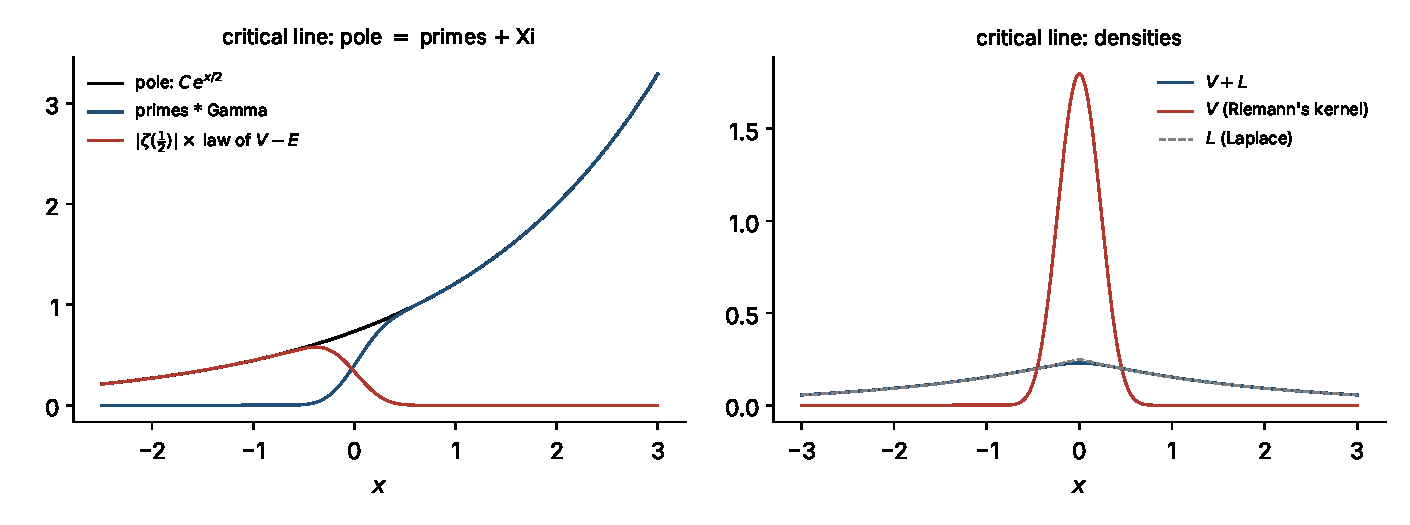
\includegraphics[width=\textwidth]{fig/v3/nk2_fig_strip.pdf}
\caption{Critical line, $\sigma=\frac12$ (computed; the letter $V$ in the figure is the variable $X$ of this chapter). Left: the pole $Ce^{x/2}$ is the sum of the prime and Gamma measure (to the right) and $|\zeta(\frac12)|$ times the law of $X-E$ (to the left). Right: densities of $X$, of the Laplace variable $L$, and of $X+L$.}
\label{nf:fig:strip}
\end{figure}

On the line the two exponentials of Nakamura's grouping combine into a Laplace variable $L$ of scale $2$, and the multiplicative form survives with $L$ on the other side.
\begin{theorem}[proved]\label{nf:thm:line}
$X+L$ has the density
\[
\frac{e^{-|x|/2}-2e^{|x|/2}\,\omega(e^{2|x|})}{|\mathcal L(\frac12)|},\qquad\mathcal L(\tfrac12)=\pi^{-1/4}\Gamma(\tfrac14)\zeta(\tfrac12)=-3.97697,
\]
and characteristic function $\mathcal L(\frac12-it)/\mathcal L(\frac12)$.
\end{theorem}

\begin{proof}
Riemann's formula $\mathcal L(s)=\int_1^\infty\omega(y)(y^{s/2}+y^{(1-s)/2})\frac{dy}y-\frac1s-\frac1{1-s}$ at $s=\frac12+it$, with $y=e^{2x}$ and $\frac1{s(1-s)}=\int e^{-|x|/2}\cos(tx)dx$; compare \eqref{riemanncont:eq:riemann}.
\end{proof}

The density is a Laplace density with a theta correction removed from its centre. Its value at the origin is $0.229714$, the total mass is $1$ to six digits, the smallest value on $[0,30]$ is $7.7\times10^{-8}$ at $x=30$, and the characteristic function at $t=3.3$ is $0.0174098584$ (computed). Since $L$ is Brownian motion at an exponential time, this is the unconditional statement that the completed zeta function on the line is a Wald side variable plus an independent Brownian side one.

Nakamura's criterion, that RH is equivalent to the survival of the signed L\'evy representation at every level of $(\frac12,1)$, sits between these statements. The densities continue into the strip without difficulty; what requires RH is the L\'evy and Thorin structure, that is, the Wald partner $T^\circ_\sigma$ of the ladder. The table of sizes shows why: at $\sigma=1.5$ two variables of variance about $4$ differ by one of variance $0.046$, and at $\sigma=1$ both are infinite.

\section{The strip law: shape, Thorin measure, zeros}\label{nf:sec:shape}

The law of Theorem~\ref{nf:thm:strip} exists for every $0<\sigma<1$ and is explicit. Write $\lambda=1-\sigma$ and $a=\sigma-\frac12$, so that $\tilde V_\sigma-E_\lambda$ has characteristic function $\mathcal L_1(\sigma-it)/\mathcal L_1(\sigma)$.

\begin{proposition}[positivity proved, log concavity conditional]\label{nf:prop:shape}
For $0<\sigma<1$ the density of $\tilde V_\sigma-E_\lambda$ is
\[
f(x)=\frac1{|\zeta(\sigma)|}\Big(C_\sigma e^{\lambda x}-g_\sigma(x)\Big).
\]
It is strictly positive (proved). As $x\to-\infty$ it is $C_\sigma e^{\lambda x}/|\zeta(\sigma)|$ up to a doubly exponentially small term, which is the pole, and as $x\to\infty$ it decays like $e^{(3-\sigma)x}\exp(-\pi e^{2x})$, which is the theta function. Its mean is $-\mathcal L_1'/\mathcal L_1(\sigma)=-\xi'/\xi(\sigma)-1/\lambda$. It is log concave, hence has a single mode, if $\log\Phi(\sqrt t)$ is concave and $\Phi$ decreasing on $(0,\infty)$, as in the statement of \cite{CNV86} discussed before Section~\ref{kr:sec:ladder} (conditional).
\end{proposition}

\begin{proof}
In the variable $y=e^{-2x}$ the density is a positive multiple of $y^{\sigma/2+1}h'(y)$ with $h(y)=\omega(y)-\frac1{2\sqrt y}$, by an integration by parts in $\mathcal L(s)=\int_0^\infty y^{s/2-1}h(y)dy$, valid for $0<\re s<1$. So positivity says that $h$ increases. By the theta inversion $h'(y)=y^{-5/2}\sum_n(\pi n^2-\frac y2)e^{-\pi n^2/y}$, positive term by term for $y\le2\pi$; for $y\ge2\pi$, $h'(y)=\frac14y^{-3/2}-\sum\pi n^2e^{-\pi n^2y}\ge\frac14y^{-3/2}-2\pi e^{-\pi y}>0$. The tails are read from the two forms of $h'$. For log concavity, $f_{\tilde V_\sigma}$ is an exponential tilt of $\Phi$, a tilt keeps log concavity, the exponential density is log concave, and by Pr\'ekopa's theorem \cite{Prekopa73} so is the convolution. This uses the concavity of $\log\Phi$, which is the unchecked statement.
\end{proof}
% UNCHECKED: the statement of CNV86 (concavity of log Phi(sqrt t)) and the monotonicity of Phi on x>0 are not verified against the paper; same status as the remark before kr:sec:ladder in ch/nc_v3_kolm.tex.

Under the hypothesis, log concavity does not depend on $\sigma$: in $u=\log y$ it says that $h'(e^u)$ is log concave, one statement about the theta function. On a grid the second differences of $\log f$ are nonpositive (zero up to rounding on the left, where $\log f$ is linear), the mode is at $x=-0.385$, $-0.460$, $-0.535$ for $\sigma=\frac12,\frac34,0.9$, and the means are $-2.00000$ at $\sigma=\frac12$ and $-4.01155$ at $\sigma=\frac34$, as the formula gives (all computed).

The Thorin measure of the strip law is the Hadamard product read through the sine squared lemma. By Theorem~\ref{thm:poisson} and Proposition~\ref{prop:struct} the strip density of $\xi$ is a sum of Cauchy bumps at the zeros, one of width $\sigma-\beta$ and mass one at each zero $\rho=\beta+i\gamma$, and the mass on $[0,R]$ is Theorem~\ref{dz:thm:mass} (with no zero on the segment from $\sigma$ to $\sigma+iR$). What the pole of $\mathcal L_1$ adds is one bump at the origin.

\begin{theorem}[Thorin measure of the strip law]\label{nf:thm:stripthorin}
Let $0<\sigma<1$, $\lambda=1-\sigma$, and put, for $v\ge0$,
\[
\kappa_\sigma(v)=\frac1\pi\re\frac{\mathcal L_1'}{\mathcal L_1}(\sigma+iv)=\frac1\pi\Big[\sum_\rho\frac{\sigma-\beta}{(\sigma-\beta)^2+(v-\gamma)^2}+\frac\lambda{\lambda^2+v^2}\Big],
\]
the sum over all zeros $\rho$ of $\xi$ (proved, from the Hadamard product, absolutely convergent). For $\Theta<\sigma<1$ the signed L\'evy measure of $\tilde V_\sigma-E_\lambda$ exists (Proposition~\ref{bp:prop:below}), and by \eqref{eq:sin2} its uncompensated Thorin measure in the chart $z=v^2$ has density $\kappa_\sigma(v)\,dv$. It is a sum of Cauchy kernels, one at each zero, positive if the zero is to the left of $\sigma$ and negative if it is to the right, and one at the origin of width $\lambda$ and mass $\frac12$ on $v>0$, from the pole. The compensated density is
\[
\kappa_\sigma(v)-\kappa_\sigma(0)=k_\sigma(v)-\frac{v^2}{\pi\lambda(\lambda^2+v^2)},
\]
the rung of Xi, \eqref{n:eq:k}, minus the Thorin density of the exponential.
\end{theorem}

\begin{proof}
The Hadamard product gives $\re\xi'/\xi(s)=\sum_\rho\re\frac1{s-\rho}$, and $-\re\frac1{s-1}=\frac\lambda{\lambda^2+v^2}$ at $s=\sigma+iv$. For the last display the exponential has $x\,m(dx)=e^{-\lambda x}dx$ on $x>0$, so the sine squared lemma gives $\frac1\lambda-\frac\lambda{\lambda^2+v^2}=\frac{v^2}{\lambda(\lambda^2+v^2)}$, and it enters with a minus sign because $E_\lambda$ is subtracted.
\end{proof}

For $\Theta<\sigma<1$ the L\'evy measure itself is Proposition~\ref{bp:prop:below}, with the additional piece $-e^{\lambda x}dx$ of the exponential on $x<0$. On the right the exponential grows and is cancelled by the primes, and what is left is $e^{-\sigma x}d(\psi_C(e^x)-e^x)$, with $\psi_C$ Chebyshev's function: the error term of the prime number theorem damped by $e^{-\sigma x}$. The integral converges on the rung $\sigma$ exactly when the error is small enough, $\sigma>\Theta$.

Under RH and for $\frac12<\sigma<1$ the picture is this. The zeros give bumps of width $a$ at their heights, the pole a bump of width $\lambda$ at the origin, and $a+\lambda=\frac12$. As $\sigma$ decreases to $\frac12$ the bumps of the zeros sharpen to atoms and the measure tends to the comb $\sum\delta_\gamma$ in $v$ (the atoms $\gamma^2$ in $z$) plus a Cauchy bump of width $\frac12$. As $\sigma$ rises to $1$ the pole sharpens to an atom at the origin, the exponential leaving to infinity, and the zeros spread to width $\frac12$. Above $\sigma=1$, \eqref{n:eq:pieces} reads $\pi k_\sigma+R_\sigma=P_\sigma+A_\sigma$, a sum of positive terms; in the strip the compensated density of Theorem~\ref{nf:thm:stripthorin} is $\pi(\kappa_\sigma-\kappa_\sigma(0))=\pi k_\sigma+R_\sigma$ with $R_\sigma<0$ continued. This is Theorem~\ref{nf:thm:strip} on the Thorin side.
\begin{figure}[t]
\centering
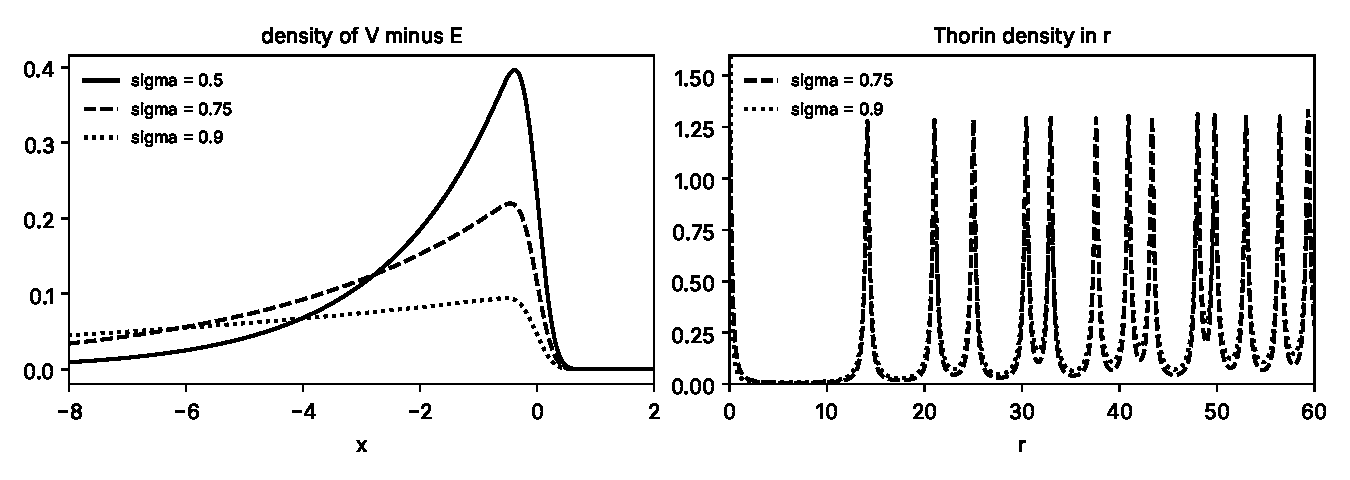
\includegraphics[width=\textwidth]{fig/v3/nk2_fig_strip_thorin.pdf}
\caption{Computed. Left: the density of $\tilde V_\sigma-E_{1-\sigma}$ at $\sigma=\frac12,\frac34,0.9$. Right: its uncompensated Thorin density in $v$, $\kappa_\sigma(v)$, at $\sigma=\frac34$ and $0.9$, with the bump of the pole at the origin and those of the zeros at $14.13$, $21.02$, $25.01$ and so on.}
\label{nf:fig:strip2}
\end{figure}

\begin{remark}[conditional (RH)]\label{nf:rem:comb}
For $\mathcal L(s)=\pi^{-s/2}\Gamma(\frac s2)\zeta(s)$ the two poles cancel on the line, $\re\frac1s+\re\frac1{s-1}=0$ at $s=\frac12+iv$. Under RH the uncompensated Thorin measure of $X+L$ is the comb $\sum_{\gamma>0}\delta_{\gamma^2}$ and nothing else, the same as for $X$.
\end{remark}

We checked the bump formula and the limit formula numerically (computed). At $\sigma=\frac34$ and $0.9$ the direct value of $\re\,\mathcal L_1'/\mathcal L_1(\sigma+iv)$ and the sum of bumps over the $1545$ zeros below height $2030$, taken over both signs of $\gamma$, agree to $2.7\times10^{-4}$ and $4.3\times10^{-4}$ at eight values of $v$, the difference being the tail of the sum; at $\sigma=\frac12$, away from the zeros, the direct value is the bump of the pole alone, for instance $0.4$ at $v=1$, and $\re\,\mathcal L'/\mathcal L(\frac12+iv)$ vanishes to working precision. For the L\'evy measure with the sharp cut $X=2\times10^7$ at $\sigma=\frac34$, the limit formula of Proposition~\ref{bp:prop:below} for the compensated value $D=\pi(\kappa_\sigma(v)-\kappa_\sigma(0))$ gives $-3.7616$, $-3.9849$, $-3.9500$ at $v=1,5,17.5$ against the exact $-3.7646$, $-3.9884$, $-3.9534$. At the first zero it gives $-0.0509$ against $+0.0066$, and the error term of the explicit formula predicts $-X^{-a}/a=-0.0598$ from that zero alone. At $\sigma=0.9$ the agreement is $2.5\times10^{-4}$ to $2.8\times10^{-4}$ away from the zeros and $2.8\times10^{-3}$ at the first zero.

\medskip\noindent\emph{Does the strip law have zeros?} There are four answers.
\begin{itemize}
\item The density has none (Proposition~\ref{nf:prop:shape}).
\item The characteristic function $\mathcal L_1(\sigma-it)/\mathcal L_1(\sigma)$ vanishes at $t=-\gamma+i(\beta-\sigma)$ for each zero, so it has a real zero exactly when $\zeta$ has a zero on the line $\re s=\sigma$. At $\sigma=\frac12$ it vanishes at every $\pm\gamma$, and for $\frac12<\sigma<1$ it has no real zero under RH, when its zeros lie on the line $\mathrm{Im}\,t=\frac12-\sigma$. This is why the law is not infinitely divisible on the line and is pretended infinitely divisible, with infinite positive mass of the signed measure away from $0$ (Proposition~\ref{sb:prop:qid}), off it.
\item The uncompensated Thorin density has no zero under RH, being a sum of positive kernels. On $0<v\le60$ the minimum of $\re\,\mathcal L_1'/\mathcal L_1$ is $0.021$ at $\sigma=\frac34$ and $0.025$ at $\sigma=0.9$, so that of the density $\kappa_\sigma$ is $0.0066$ and $0.0080$ (computed).
\item The compensated density does change sign, and how depends on the height. The compensator is $\kappa_\sigma(0)\pi=\xi'/\xi(\sigma)+1/\lambda=:c$, while the average of $\re\,\mathcal L_1'/\mathcal L_1(\sigma+iv)$ over $v$ near $R$ is $\frac12\log\frac R{2\pi}$. At low height the density is positive only in a window around a zero, where the bump has height about $1/a$, and this needs roughly $1/a>1/\lambda$, that is $\sigma<\frac34$: on $0<v\le60$ there are $26$ sign changes at $\sigma=\frac34$, a small window around each of the $13$ zeros, and none at $\sigma=0.9$ or at $\sigma=\frac12$ off the atoms (computed). On every rung the zeros outweigh the pole in the end. The cumulative statement, that the compensated mass on $[0,R]$ changes sign near $R=2\pi e^{2c+1}$, follows from the mass identity and $N(\sigma,R)=o(N(R))$. The height $R_\sigma=2\pi e^{2c}$ at which the average over windows of length $60$ crosses $c$ is a heuristic threshold. It is $941$ at $\sigma=0.6$, $1.917\times10^4$ at $\sigma=\frac34$ and $3.2\times10^9$ at $\sigma=0.9$, and tends to $2\pi e^4=343$ on the line (computed). At $\sigma=\frac34$, in windows of length $60$ around $R=1000$, $5000$, $19170$ and $60000$ the mean is $2.547$, $3.364$, $3.981$ and $4.565$ against $\frac12\log\frac R{2\pi}=2.535$, $3.340$, $4.012$, $4.582$ and $c=4.012$, and the fraction of the window on which the compensated density is positive is $0.19$, $0.34$, $0.50$ and $0.64$ (computed).
\end{itemize}
None of this locates a zero. Theorem~\ref{nf:thm:stripthorin} is the Hadamard product read through the sine squared lemma, and positivity of its uncompensated measure on the rung $\sigma$ is the statement that no zero lies to the right of $\sigma$. The pole becomes a visible, positive, explicit piece of the Thorin measure in the strip, where above $\sigma=1$ it was a variable to be divided out.

\section{What the factorisation gives}\label{nf:sec:gives}

The factors of Nakamura's measure are identified in three languages.
\begin{center}
\small
\begin{tabular}{llll}
\toprule
& in $t$ (Nakamura) & in $u$ (Thorin) & hitting time\\
\midrule
primes & $\log N_\sigma$, zeta law & $T^P_\sigma$ & first passage to $\log N_\sigma$\\
Gamma & log gamma & Bondesson's term & $B$ at the time $X_a$, $a=1+\frac\sigma2$\\
pole & exponential & reciprocal gamma & last exit, Bessel(5)\\
Xi & $\tilde V_\sigma$ & $T^\circ_\sigma$ & $H=2T$ on the line, a GGC iff RH\\
\bottomrule
\end{tabular}
\end{center}
It is not a path to RH. The multiplicative factorisation lives where the Euler product converges. Its additive continuation into the strip (Theorem~\ref{nf:thm:strip}) is the functional equation and carries no information about zeros. Corollary~\ref{nf:cor:transport} rests on Proposition~\ref{bp:prop:valpha}. On the critical line the Wald partner exists unconditionally, and only the statement that it is a generalised gamma convolution is equivalent to RH. What the factor by factor reading adds is the classification by sides, which says why no single factor can be continued: the pole and the Gamma factor are on the Brownian side for every $\sigma$, the primes are on neither, and only the full quotient lands on the Wald side.

\begin{problem}
Give Nakamura's density of $\tilde V_\sigma$ a pathwise form compatible with Theorem~\ref{nf:thm:four}: a coupling in which $\tilde V_\sigma+E_{\sigma-1}$ and $\log N_\sigma+L_\Gamma$ are equal, not only equal in law.
\end{problem}
\begin{problem}
In Nakamura's grouping the Gamma factor on the rung $\sigma$ is $B_{X_{\sigma/2}}$. The zeros of the Mellin transform of $X_\lambda$ are expected on one line at $\lambda=\frac12$ (the Riemann hypothesis for $L(s,\chi_4)$, not known) and lie on two lines at $\lambda=1$ (Chapter~\ref{ml:ch:mellin}), that is, at $\sigma=1$ and $\sigma=2$. Is there a reason in the factorisation for these two rungs?
\end{problem}
\begin{problem}
Is there a symmetric variable built from the primes that lies on the Wald side? By the table $\log(N/N')$ does not. The completed function on the line, $X+B_e$, mixes sides; find its decomposition into a Wald part and a Brownian part without using the zeros.
\end{problem}
\begin{problem}
Prove directly, from the first passage identities of Section~\ref{nf:sec:wald}, that $T^{\mathrm{pole}}_\sigma$ is a convolution factor of $T^P_\sigma+T^\Gamma_\sigma$ for $\sigma>1$, without Proposition~\ref{bp:prop:valpha}.
\end{problem}

\section{What this leaves open}\label{n:sec:path}

The positivity results that the draft derived at length are in the book in stronger form and are only listed here. Positivity of $k_\sigma$ for every $\sigma\ge1$, strictly, is Propositions~\ref{bp:prop:v1min} and \ref{bp:prop:valpha} (ball arithmetic). On RH the strict positivity for every $\sigma>\frac12$ is Theorem~\ref{yo:thm:coercive}, with the gap bound of Lemma~\ref{yo:lem:gap}. The unconditional ranges and the window $0<|v|\le3\times10^{12}-1.21$ are Theorem~\ref{thm:dbeta:minall}. The equivalence of RH with positivity at every level of the strip is Theorem~\ref{cx:thm:rhmin}, and the analogue for $\chi_4$ is Theorem~\ref{thm:dbeta:minall}(vi). The minimum of $v_\sigma$ at the origin on RH, for every $\sigma>\frac12$, and unconditionally for large $\sigma$, is the theorem of Lagarias \cite{Lagarias}. Garunk\v{s}tis \cite{Garunkstis02} extended the unconditional statement to every zero free half plane, which by the theorem of \cite{OAI26a} (Section~\ref{qrh:sec:claims}) gives every $\sigma>\frac78$ (proved).

Three statements about the reciprocal at the levels of the strip are each equivalent to RH, when asked for every level of $(\frac12,1)$: the pretended infinite divisibility of Theorem~\ref{n:thm:nak}, the existence of the Thorin representation, and the positivity of $k_\sigma$. Each is a statement about the whole family of levels tending to $\frac12$. A single level $\sigma<1$ is weaker: a zero free half plane $\re s>\sigma$ is not RH. The sine squared lemma and Bochner's theorem translate one equivalent form into another, the criteria of Pólya and Gneiting are only sufficient, and none of them carries information about where the zeros are.

Why positivity does not descend for free. When a representation exists at level $\sigma-\varepsilon$, \eqref{n:eq:kzero} gives
\[
k_\sigma+\frac{c_\sigma}\pi=P_\varepsilon*\Big(k_{\sigma-\varepsilon}+\frac{c_{\sigma-\varepsilon}}\pi\Big).
\]
Smoothing by $P_\varepsilon$ preserves positivity and moves upward in $\sigma$. Descent needs the inverse, Poisson deconvolution, which does not preserve positivity and is ill posed. A route through this chapter would have to show that the deconvolution of $k_\sigma$ by $P_\varepsilon$ stays a positive measure plus a constant for every $\varepsilon<\sigma-\frac12$, starting from $\sigma>1$, where positivity is known. This is the Thorin ladder of Volume I. One place for new input is the prime side: lowering $\sigma$ multiplies the prime atoms by $n^\varepsilon$, and \eqref{n:eq:primecond} must then be maintained by $\Delta(X)=\psi(X)-X$ at the new level. A bound on the cosine transform of $\Delta$ stronger than any zero free region gives would push the absence of zeros below the line $\re s=1$. This is a statement about the primes alone (heuristic as a programme, open). The chapter reaches no such bound and claims no route to RH.
